\chapter{Preliminary Actions I: Biosensing and Actuation Couplings}
\label{cha:Preliminary_Actions_sens_act}

Our first research actions were lab-based, first-person experimentations  with biofeedback. From this, we developed a strong understanding of the expressive affordances of physiological modalities. Here, we report our initial findings as a series of conceptual use-cases in context of a review article that was delivered during the doctorate programme, including personal contributions as respective co-authors.

\printpublication{alfaras_biosensing_2020}

% Alfaras, M.; Primett, W.; Umair, M.; Windlin, C.; Karpashevich, P.; Chalabianloo, N.; Bowie, D.; Sas, C.; Sanches, P.; Höök, K.; Ersoy, C.; Gamboa, H. Biosensing and Actuation—Platforms Coupling Body Input-Output Modalities for Affective Technologies. Sensors 2020, 20, 5968. https://doi.org/10.3390/s20215968

% \section{Biosensing and Actuation Couplings: An Overview of Concepts and Technical Resources}

\section{Introduction}

In this Section, we present an overview of biosignals that have become standard in low-cost physiological monitoring and show how these can be matched with interaction design concepts for facilitating \textit{bodily engagement} and \textit{aesthetic experiences}. First-person soma design lets researchers look afresh at biosignals that, when experienced through the body, are called to reshape affective technologies with novel ways to interpret biodata, feel it, understand it and reflect upon our bodies. Taking both strands of work together offers unprecedented design opportunities that inspire further research. Through first-person design, an approach that draws upon the designer’s felt experience and puts the sentient body at the forefront, we outline a comprehensive work for the creation of novel interactions in the form of couplings that combine biosensing and body feedback modalities of relevance to affective health. These couplings lie within the creation of design toolkits that have the potential to render rich embodied interactions to the designer and user alike. As a result we introduce the concept of “orchestration”. By orchestration, we refer to the design of the overall interaction: coupling sensors to actuation of relevance to the affective experience; initiating and closing the interaction; habituating; helping improve on the users’ body awareness and engagement with emotional experiences; soothing, calming, or energising, depending on the emotional and social context and the intentions of the designer. The findings of these explorations are moralised as a set of experimental sensor-actuation couplings to gain a broader perspective on designing embodied systems.

% Moved to chapter 2
% \subsection{Somaesthetic Design in Practice}
%
% We take somaesthetic design—a design stance that draws upon the felt body and takes inspiration from experiencing it—and then combine it with the innovative integration of biosensors and actuators. The disruptive somaesthetic view, moves away from the idea of monitoring the body for the sake of bad habit reduction in pursuit of a healthy and long life \cite{hook_somaesthetic_2015}. Soma design, rather, lets us get attuned to our bodies and use sensations as a valuable resource instead of something to be improved to meet performance standards. In this context, we present novel research on embodied interaction design couplings, that is, sensing-actuation combinations of aesthetically evocative body input-output modalities that render biodata shareable, body-centered, highly tangible or even able to be experienced collectively.
%
% With a focus on the body, design research is used as a way to enter introspectively to emotional self-reflection and potentially disrupt the way we relate to our mental well-being with technology-mediated interactions. Technology-mediated interactions, drawing upon ubiquitous computing capabilities could add novelty and be taken further to psychotherapy contexts. Using technology for sensing and actuating upon our body, we can get access to bodily states from our physiology to then act in such a way that we help to alter or reassess our psychophysiological states. This construction process may be developed to extend our knowledge and expectations regarding the internal mechanics of our own body and serves as a bridge to design better informed affective health technologies. This comprises the first-person design stance, the somaesthetic design (“design with the body”) approach \cite{hook_designing_2018}, and the path to orchestration.

\section{Sensing Strategies}
\label{sec:sensing}

Physiological signals are time representations of changes in energy produced in the body (see Section \ref{subsec:physiological_sensors}). These changes correspond to energy variations of different nature, such as electrical, chemical, mechanical, and thermal \cite{semmlow_biosignal_2014}. Through digitization, these serve as a somatic input of an interactive artefact, processing new data while it is running, thus enablimg a unique and continual engagment with its aesthetic parameters \cite{carvalhais_art_2022}. Here, we present a selection of wearable sensors that can be incorporated into the creation of novel communication systems. In particular, we will focus on a subset of sensing modalities compatable with the R-IoT module (described in Section \ref{subsec:riot}), offering a brief description of the physiological process, common feature extraction methods, suitable placement on the body and assess some of the challenges of signal artifacts that arise during movement.

\begin{figure}[htbp]
\centering
\includegraphics[width=0.75\linewidth]{Chapters/Figures/preliminary_actions/biosignals_actuation/signals_ACC.png}
\caption{Visual representation of different physiological signals: (a) Respiration, (b) Electromyography (EMG) and (c) Inertial Measurement Unit (IMU)}
\label{fig:biosignals_samples}
\end{figure}

% We present a collection of embodied sensors that have been addressed in our research. The following offers a brief description of the physiological process, common feature extraction methods, suitable placement on the body and assess some of the challenges of signal artifacts that arise during movement.
% This democratization of the study of biosignals comes with interesting possibilities such as a better understanding of the self and a richer, unprecedented way to interact with technologies that accompany us. This yields an opportunity to define alternative ways to live an affectively healthy life.

\section{Respiratory Sensing}
\label{sec:respiratory_sensing}

Respiration sensors monitor the inhalation-exhalation cycles of breathing, i.e. the process to facilitate the gas exchange that takes place in the lungs. In every breathing cycle, the air is moved into and out of the lungs. A breathing sensor uses either piezoelectric effects on bendable wearable bands or accessories (one of the most predominantly used technologies), respiratory inductance plethysmography on wired respiration bands around the thorax, microphones on the nose/mouth airflow, plethysmographs (measuring air inflow) or radiofrequency, image and ultrasonic approaches. A review on breathing monitoring mechanisms is found at \cite{massaroni_contact-based_2019}. For piezoelectric breathing sensors, thoracic or abdominal displacements produced in breathing cycles bend a contact surface that converts ressistive changes to continuous electrical signals
(see Figure \ref{fig:biosignals}a).

A piezoelectric breathing sensor is usually located on the thoracic cavity or the belly, using a wearable elastic band. With adjustable strap and fastening mechanisms, the sensor can be placed slightly on one side where bending is most relevant, optimizing the use of the sensor range. These kinds of sensors, allow both the study of thoracic and abdominal breathing. With the development of conductive fabric, breathing sensors are making its way into the smart garment market in the form of T-shirts and underwear bands. Breathing is a relatively slow biosignal, with breathing rates often below 20 inhale/exhales per minute. A sampling rate frequency as low as 50Hz is sufficient to capture the dynamics of respiration.

A breathing signal informs the respiration dynamics of the subject, i.e. the dynamics of the process mediating gas exchange in the lungs. The monitoring of an innate breathing action brings in the assessment of breathing cycles and rates which can be used to handle problems involving breathing interruptions, oxygen intake, metabolism of physical activity, as well as emotional stressors. In terms of analysis, breathing cycles are studied using breathing rates, the maximum relative amplitude of the cycle, inhale-exhale volume estimation, inhale-exhale duration, and inspiration depth, that allow the characterisation of several breathing patterns.
% From an incoming data stream, it's possible to discern the Respiration rate, Inspiration duration expiration duration, Inspiration-expiration ratio, and Inspiration depth.

While piezoelectric breathing sensors are prominent given the low cost and form factor advantages of wearable sensor platforms, deviations in placement have an effect in the relative range of the response signal. Movement artefacts, most relevant when physical activity is present, are a common source of problems. Respiration sensing techniques like the respiratory inductance plethysmography, compensate the highly localised piezoelectric approach with a sensor capturing the general displacement of the whole thoracic cavity, yielding a signal less prone to movement artefacts. The monitoring of breathing cycles is usually accurate, although the exploration of effects to be used as voluntary inputs in interactions, such as holding the breath, are not easily captured.

\section{Surface Electromyography (sEMG)}
% \noindent \textbf{How it works:}
The recording of the electrical activity produced by skeletal muscles receives the name of electromyography (EMG). Human muscles are made up of groups of muscle units that, when stimulated electrically by a neural signal, produce a contraction. The recording of the electrical activity of the muscles (voltage along time), traditionally relying on intrusive needle electrodes (intramuscular), is easily accessible nowadays by means of surface electrodes that capture the potentials of the fibers they lay upon. The result of this measurement is a complex surface electromyography signal (sEMG) that reveals data about movement and biomechanics of the contracted muscles.
(see figure \ref{fig:biosignals_samples}b).

% \noindent \textbf{What:}
Electromyography signals inform about the contraction of specific muscles and parts of the body. The EMG signal consists in the time representation of rapid voltage oscillations. Its amplitude range is approximately 5mV. The EMG signal grants an assessment of several aspects of a physical activitys such as muscle contraction duration, the specific timing at which movements or contractions are activated, the presence of muscular tension or fatigue, and the extent to which different fibers (area) are contracted. The analysis is conducted through noise filtering, together with feature extraction that yields contraction onset detection, the estimation of signal envelopes, and the computation of average frequencies.This lets subjects deepen their understanding of movement strategies, very relevant for embodied art and sports performance, improve muscle coordination, or even reveal existing movement patterns that they are unaware of.

% \noindent \textbf{Features:} Onset instants; Max amplitude; Instant of maximum amplitude; Activation energy; Envelope;
% \noindent \textbf{Where:}
Having become the standard in EMG monitoring, bipolar surface electrodes consist of three electrodes. Two of them (+/-) must be placed close to each other, on the skin that lies on top of the muscle under study, along the fibers' direction, while the third one is placed in a bony area where no muscular activity is present. This allows the measurement of electrical potential differences with respect to a common reference, yielding a unique signal that represents the muscular activity of the area. Given the fast muscle-neural activation nature of EMG signals and the presence of different active muscles contributing to the same signal, muscle activity must be acquired at sampling rates no lower than 200Hz frequencies. Working at 500Hz is desirable, while a sampling rate of 1000Hz guarantees the tracking of all the relevant events at a muscular level.

Surface EMGs are intrinsically limited to the access to superficial muscles. This is compromised by the depth of the subcutaneous tissue at the site of the recording which depends on the weight of the subject, and cannot unequivocally discriminate between the discharges of adjacent muscles.
Proper grounding (reference electrode attached to a bony inactive muscular region) is paramount to obtain reliable measurements. Motion artifacts and muscular crosstalk compromise the assessment of the muscle activity under study. In this context, interference from cardiovascular activity is not uncommon, particularly in areas such as chest and abdomen. sThe presence of power supplies and mains (powerline) in the vicinity poses the risk of 50Hz-60Hz interference.

% Movement - inertial and environemtal
\subsection*{Inertial Measurement Unit (IMU) signals}
% \noindent \textbf{How it works:}
An inertial measurement unit (IMU) combines accelerometers, gyroscope, and magnetometer sensors to measure acceleration, rotation, and magnetic field in the three spatial directions. Used as a body sensor, it informs about its movement. Built upon microelectromechanical systems (MEMS), accelerometers use the displacement of a tiny mass surrounded by capacitors to measure proper acceleration. Gyroscopes, use the Coriolis displacement of two opposite oscillating masses to measure the rate of rotation (or rotation speed). Magnetometers are capable of measuring the surrounding magnetic field by means of magnetoresistance changes, informing about the orientation. Hence, IMU signals depict voltage variations corresponding to acceleration changes measured by accelerometry (ACC), rotational speed changes measured through gyroscopes (GYR) and magnetic field fluctuations measured by magnetometers (MAG), throughout a given dimension in space
(see Figure \ref{fig:biosignals}c).

% \noindent \textbf{What:}
IMU signals inform about the properties of the movement of the body which they are attached to, such as orientation and changes in speed. The measurement of accelerations and rotations, together with orientation, helps the researchers assess the existing movement patterns. Characteristics such as tilt (orientation), changes of direction, or number of repetitions in a given movement pattern (e.g. steps) are usually addressed. This makes possible the understanding of gait, posture, the dynamics of specific gestures or movements, as well as the detection of undesired movement patterns. Moreover, the measurement of movement properties is crucial in areas like ergonomics research and in estimating the metabolic equivalent of tasks addressed in physical effort studies.
% In terms of features and processing, information of interest can be fundamental frequencies or rates, maximum angles (movement range), and maximum accelerations are of interest.

% \noindent \textbf{Features:} Metabolic equivalent of task (MET); Angular position (with respect to the ground plane); Footstep instants; Maximum acceleration; Maximum angular velocity. More advanced processing of multiple sources integrated can delve into gesture recognition, gait assessment, and other movement pattern analysis.

% \noindent \textbf{Where:}
The use of IMUs is very extended in monitoring navigation systems, present in many vehicles, and the devices are nowadays part of the set of sensors that mobile phones are equipped with. IMUs used as the body movement tracking systems work through the different sensors placed on the body part that is subject to study. This is typically the case of limbs and joints, shoulders, hips, or head, among others \cite{niswander_optimization_2020}. Just like in the case of mobile phones, the wide use of IMUs has fostered the appearance of gadgets and wearables equipped with this monitoring technology (e.g. helmets, head-mounted displays, handles, controllers, footwear) that can monitor movement properties without necessarily having to attach sensors on the body.

\section{Actuation Mechanisms}

The mechanisms to provide actuation in a form of feedback to the human take an important role in creating a complete interaction from sensing body properties to making the subject aware of them. Our research aims at linking biosensing to body actuation. Actuation is generally provided by mechanical elements that move and respond to input signals in order to either control or inform about a system. We stretch this definition to include feedback mechanisms such as screen-based visuals, although no mobile mechanical element is necessarily implied. In this section, we focus on actuation mechanisms that can be easily controlled and coupled to our body. We take a similar approach to the structure used to describe the biosignals, provding a technical overview while also explaining the actuator limitations and usage precautions for a selected list of actuators. The range of actuation mechanisms presented draws upon our research on affective technologies and interaction design, as well as inspirational works present interaction design research, but it should be seen as a non-exhaustive list of possibilities.

\subsection*{Visual Feedback}

% \noindent \textbf{How it works:}
Visual biofeedback is the representation of bodily signals over time, capable of informing physiological changes, initiated from within the body. Examples of this could be ECG feedback, respiration feedback, or movement tracking, usually employed in health metrics or sports performance research. Screen-based systems for biosensor feedback are standard practice in clinical settings and hospitals, purposed as a means to assess the dynamics of the aforementioned changes, helping to gain understanding and tracking the inner state of a given subject. Biofeedback use has for instance been adopted in psychotherapy, as research suggests that the technique provides a mechanism to self-regulate the emotions.

Screen-based visual biofeedback can be projected from a 2D graphical a display, either a computer screen or a designated sensing platform display. This modality benefits from direct control over light, colours, strokes, and visual styles to represent a changing signal that evolves with time. Signal peaks and troughs appear in an axis showing the measurement magnitude in a given range, so that rapid and slow dynamics can be seen as the representation moves along the time axis when updated.

To facilitate a live convergence between the input and feedback, it is important that the represented signals are updated in real-time. Doing otherwise, although possible using delays or technology limitations, would compromise the ability of the actuation to convey the tracking meaning attributed to the practice of biofeedback. When sensing requirements pose concerns on the technical ability to render a smooth representation through time, approaches such as averaging or undersampled representations are used.

Screen-based visual biofeedback connects easily with the mathematical properties that underlie the signals under study. However, signal processing procedures such as filtering, scaling or normalisation are crucial in achieving a smooth and flowing representation. These come, of course, tightly dependent on the available resources in computational power.
There are situations in which feedback users report finding difficulties or experiencing anxiety when engaging in the assessment of body rhythms. Moreover, visual information tends to remarkably capture the attention of the user, thus needing special care when used as an element of broader interaction (movement, performance, exercise) that could render a poorer experience quality or present a deviation from the aimed activity.

\subsection*{Sound Feedback}

Sound feedback, when applied to biosignals, is the audio representation of body signals that uses sound properties to inform about body changes happening along time. Its goal is to exploit our sophisticated trained sense of hearing to convey meanings linked to body signal features, leading to the understanding and tracking of a given subject’s biosignal dynamics.

Sound feedback uses the properties of sound, i.e. volume, pitch or frequency (note), rhythm, harmony, timbre, and transients (attack, sustain, etc.) among others, to represent a signal (or its features) that changes over time. Its generation, often using speakers or headphones, is linked to properties of the signal. Alternative approaches draw upon several transducing paradigms, i.e. different ways to convert electrical signals into sound (electromechanical as in the case of speakers, piezoelectric or others), often more limited such as buzzers or beepers made of basic vibrating elements that produce sound.

Sound can be produced by speakers when amplifying electrical pulses to audible vibrations, allowing users to listen to the feedback without the need for additional equipment. Headphones, working by the same principle, can be used for the same purpose but only providing feedback to the person wearing them. The human hearing range typically comprises frequencies between 20Hz and 20000Hz. The oscillating frequency of the sound wave that is created is what gives it a particular tone (what we call a note). The different times at which sound waves are generated is what creates the meaning of rhythm and articulation.

Audio generation and processing techniques are complex. Whilst high-level hardware and software tools can be exploited to make a complete system more accessible, there certainly remains a relevant learning-curve. The scenario in which audio feedback is deployed conditions a lot the effect achieved, given the fact that materials surrounding the sound generating system at use impose effects like reverberation, echoes, or absorption. Exposure to sound feedback for a prolonged period of time has some drawbacks. Excessive volumes can be harmful one´s auditory system, to the point of irreversible hearing impairment. Sound elements that lack textural richness (e.g. a pure sine-wave) may limit long-term engagement from users or potentially cause irritation.

\subsection*{Vibrotactile Actuation}

Vibrotactile actuation uses motors to stimulate communication utilizing touch sensitivity, and more precisely tactile vibrations. When linked to physiological sensory, the vibration feedback can be used used to convey features of the biosignal being tracked. This mechanism is built upon motors, which can mostly be categorised under two types: Eccentric rotating mass vibration motor (ERM), and Linear resonant actuator (LRA). These actuators usually enclosed within a small capsule with simple positive and negative ($+/-$) terminals to be driven. The typical power requirements for these components normally range between 1 Volts and 5 Volts.

With weights below 1g, the small form factor of these actuators makes them suitable for body explorations, often relying on patches, elastic bands, or holders. Typical uses include also vibrotactile-equipped wristbands or smartwatches. Besides the traditional game/remote controllers including vibrotactile feedback and actuating on the hands, the currently ubiquitous role of mobile phones has spread the use of vibration feedback and patterns for notification, alarms and other communication examples anywhere a phone can be placed or hold. Small vibrotactile motors feature fast startup and breaking times and can actuate taking rotations up to 11000 revolutions per minute (RPM), in the case of ERMs, and oscillations of the order of few hundreds of Hertz.

Vibration comes often with undesired noises or sounds. While this is mitigated by rubber-made absorbing structures often integrated in the motors, use cases need to consider this aspect. While vibrotactile actuation offers the opportunity to explore a particular type of haptic feedback, the use of small motors limits the generated effects, in terms of amplitude, duration, and intensity perceived. To create vibration sequences, several motors are needed, provided integration software and hardware development efforts are carried out. The actuators often require extra drivers to widen the operating regime possibilities while maintaining electrical safety standards. As generally advised in the case of feedback modalities applied to the body, haptic feedback actuation has to go hand in hand with user experience studies, since prolonged exposure and certain placements can lead to discomfort.

% \subsubsection{Temperature Actuation}

\subsection*{Shape-changing Actuation}

% \noindent \textbf{How it works:}
% \noindent \textbf{What:}
Shape-changing actuation uses interfaces that exhibit changes in size, shape, or texture in order to exploit the human visual and tactile perception to convey meanings and information content. When linked to feedback, these shape-changing mechanisms convey meanings intrinsic in the dynamics of the information that they are linked to, such as rapid changes, stability, increase, decrease, and steady growth. Such interfaces, despite the parallelisms found in visual screen-based explorations done in visual computing, are emerging as an alternative, physical, and tangible way of interacting with technological devices \cite{alexander_shape-changing_2017}.
Three of the most widely used examples of shape-changing actuation elements are Shape-memory wire (``muscle wire'', nitinol, flexinol), Linear actuator and Inflatable shapes.
% \begin{itemize}
% \item Shape-memory wire (``muscle wire'', nitinol, flexinol): a unique type of wire, which can be deformed, stretched and bent at room temperature, able to restore its shape when heated (i.e., when exposed to the electrical current). The wire activates rapidly when the electrical current is applied or the wire is heated.
% \item Linear actuator: a mechanical device that converts electrical current into a linear movement along a given axis, as opposed to the circular motion of a conventional electric motor. When equipped with extra sensors (such as Hall effect sensors) they are able to provide precise information on their length(the absolute position of the moving element on the axis).
% \item Inflatable shapes: enclosed structures which can be inflated with fluids (typically gas: air, oxygen, nitrogen, helium, etc.), usually accompanied by pressure or volume control mechanisms.
% \end{itemize}

% \noindent \textbf{Where:}
In order for the technology to best benefit from the focus on visual and tactile perception, shape-changing actuation implementations must remain under reach (sight or touch) to convey the meanings embedded in the changes of shape. This can entail direct contact with the body, with the potential to increase the felt shape meaning when in contact with a large body area, or where touch sensations are more developed, or within the field of vision of the user.

% \noindent \textbf{When:}
The wide range of shape-changing actuation possibilities comes with different actuation timings in it. While it is possible to work with shape-memory wires that are rapidly heated or compressed gas or pumps that quickly fill up a given inflatable, the time affordances of this kind of actuation do not generalize. Linear actuators, for instance, usually require a system of pistons and damping mechanisms that have an impact on the dynamics of the actuation while it unfolds over time. Moreover, it is often the case that the behavior of shape-changing interfaces is not symmetrical, for example, although an inflatable can be rapidly fed air by a pump or a reservoir, deflation valves have their own rules.

% \noindent \textbf{Limitations:}
Memory wires, although visually appealing, imply the utilization of high temperatures which challenges the use of haptic shape-changing feedback based on them. In turn, the strains achieved (or pulling forces) are generally weak, often leading to implementations that use several wires. In the case of linear shape-changing actuators, movement is often accompanied by undesired noise and relatively slow dynamics. The actuators themselves, made of rigid moving elements, impose a certain rigidity to the overall actuation. Moreover, multiple units are often needed to create appealing effects.
Shape-changing inflatables often present problems of fluid leaks, as well as different asymmetric behaviors for inflation and deflation. These can be tuned by further developments on valves and compartments but requires significant work. Besides, the type of pump poses specific fluid requirements and usually exhibits noise that interferes with the actuation designed.

\subsection*{Aesthetic Characteristics of Actuation Modalities}

Taking the aesthetic criteria set out in Section \ref{sec:aesthetic_qualities}, we breifly describe some of the spatial and rhythmic qualities of interaction that are complimentary to the actuation modalities listed above. To begin, we propose that visual feedback is well attuned to spatial aesthetic qualties, where pixel-based displays are capable of projecting highly granular representations that take upon aesthetically engaging features, such as systemtric (and asymmetric) structures. \citeauthor{li_overview_2020} provide a comprehensive review of conginitive proceses that occur when perceiving low-level visual features \cite{li_overview_2020}. In Chapter \ref{case_studies:modi_dis}, visual feedback is utilised to articulate internal sensations such as muscular activation and balance while a physical gesture is performed and presented to an audience, developed from the guidlines for visualization set out in Chapter \ref{preliminary_actions:modi_ws1}.

Sound feedback can conveniently be associated with rhythmic qualities when a regular ``pulse'' is clearly present \cite{danielsen_moving_2015}. In the following Section \ref{sec:breathing_synchrony}, we demonstrate how shared sound feedback can foster physiological entrainment between two users, sustaining synchronous inhale-exhale rhythms. Sound can indeed be used to provoke qualities of space, a clear example of this being the use of particular reverb effects to mimic the feeling of being situated in a particular space, such as a large hall. This feature is still constrained within the singular dimension of time, however. In order to achieve a sense of localisation that's authentic to three-dimensional space, the binaural arrangement of conventional listening mediums can be limited here \cite{chang_impairments_2018}. Studies into ambisonic configurations provide a promising research path, however these still retain a high barrier to use when considering cost, learning-curve and portability \cite{huisman_sound_2021}. Our Case Study III, Chapter \ref{case_studies:adse_ess} showcases an interactive framework to engage many users with one another by leveraging both rhythm and localisation with several mobile speakers.

Tactile forms of feedback, be it from vibration or shape-changing mechanisms, impose feedback directly onto the body, which can be arranged to target specific limbs, muscles, bones and organs. In terms of spatial aesthetics, these tools are resourceful for harnessing one's sense of proprioception, raising awareness to their bodily functions. Moreover, by applying shape changes that unfold over time, the actuation dynamics are brought forth letting the user be able to play with concepts such as time (increasingly/decreasingly fast, slow, abrupt) and volume or size to depict the desired information. In Chapter \ref{case_studies:soma_chi}, Section \ref{sec:aesthetic_qualities}, we go into detail of the aesthetic affordances that arise while engaging with shape-changing materials over prolonged assessment period. In this case, we study how symmetry, synchrony and bodily alignment can influence one's habitual respiratory rhythm and posture.

\subsection*{Orchestration}

% By orchestration, we refer to the design of the overall interaction: coupling sensors to actuation of relevance to the affective experience; initiating and closing the interaction; habituating; helping improve on the users' body awareness and engagement with emotional experiences; soothing, calming, or energising, depending on the affective health condition and the intentions of the designer.
By orchestration, we refer to the design of the overall interaction: coupling sensors to actuation of relevance to the interaction space; initiating and closing the interaction; habituating; helping improve on the users' body awareness and articulation of emotion. Such mechanisms try to achieve the overarching goal of linking body measurements to meaningful representation through actuation that addresses various modalities that act on our bodily senses, be it visual, hearing, touch or otherwise. To achieve this facilitation it is crucial to be able to combine and nicely coordinate the relationship between input (sensors) and output (actuators). In this scope, the term orchestration defines the process of:
\begin{itemize}
    \item Creating couplings, that is, combining biosensors and actuators in place
    Coordinating the technology-mediated body interactions
    \item Working on the sequence in which different modalities are addressed via the sensors and actuators. Deciding which one goes first
    \item Understanding the design possibilities, acknowledging affordances, limitations and roles of the involved technologies that involved in these interactions
    \item Consolidate the process of introducing a new user to the experience, defining a balance between explicit interaction or open exploration
    \item Retrieving meaning information from the input data, potentially laying out machine learning, feature extraction, smart event recognition, or signal processing tools that can be applied to render the interactions more intuitive
\end{itemize}

\section{Breathing in Synchrony: From Physiological Synchrony to Audio Feedback}
\label{sec:breathing_synchrony}

Taking the orchestration principles described above, we present a preliminary coupling. This example draws upon the psychology concept of therapeutic alliance \cite{koole_synchrony_2016}, takes respiration data from two users in the same physical space, each equipped with personal wearable devices that stream data wirelessly to a host computer. In this example, two users participate in a timed breathing exercise together whilst their individual respiratory patterns are being measured with piezoelectric (PZT) bands placed around the diaphragm (see Figure \ref{fig:breathe}). The data is aggregated on the host computer, executing a script that measures the collective breathing activity. From here, we apply shared biofeedback in the form of sound to stimulate synchrony awareness and physiological dialogue between users over time.

\begin{figure}[htbp]
\centering
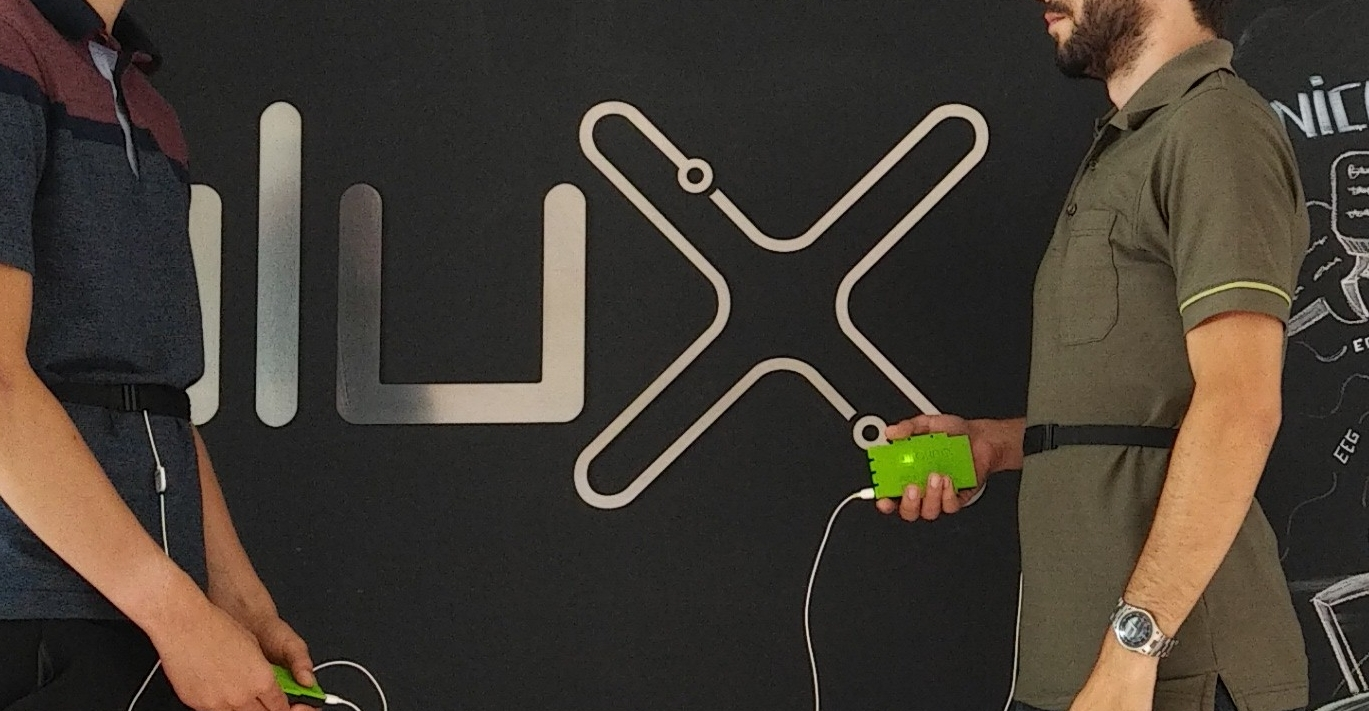
\includegraphics[width=0.7\linewidth]{img/breathe_sync.jpg}
\caption{Breathing synchrony-audio experiment, based on the analysis of two piezoelectric abdominal respiration signals}
\label{fig:breathe}
\end{figure}

\subsection*{Synchrony as a Basis for Collective Engagement}

Synchrony in neural and physiological activity has been hypothesised to be a mechanism for empathy, mutual understanding, and trust \cite{wallot_beyond_2016}. It can describe a rhythmic coordination of movements and biological behaviour to an external signal \cite{koole_synchrony_2016}. Synchrony can be present in different relational contexts, such as therapist to patient \cite{koole_synchrony_2016}, couples \cite{karvonen_sympathetic_2016}, close friends \cite{miles_birds_2011}, as well as mother and child \cite{butler_emotional_2013}. Synchrony have certain positive effects on individual’s well-being. For example, leading people to synchronous movements facilitate cooperative behaviour \cite{kirschner_joint_2010}, potentially linked to increases in self-esteem, compassion and rapport \cite{lumsden_sync_2014, fujiwara_rhythmic_2020}, moving in synchrony also leads participants to greater perceptual sensitivity to movements \cite{zamm_endogenous_2016}.

\subsection*{Respiration as an Expressive Indicator}

While searching for practices beneficial for affective well-being, breathing exercises were also considered. Recent research indicates that many of the detrimental effects of negative emotional states and sympathetic dominance of the autonomous nervous system can by counteracted by different forms of meditation, relaxation, and breathing techniques. In fact, meditation and breathing techniques can reduce stress, anxiety, depression, and other negative emotional states \cite{brown_sudarshan_2005,descilo_effects_2010,regulation_2015}. Moreover, body-centred practices, such as dance or martial arts, require coordinating breathing patterns not only with our own movements but also the person we are moving with \cite{codrons_spontaneous_2014}.

\subsection*{Sensory Input and Processing Strategies}


The exploration followed a stage of preliminary research on physiological synchrony features drawn from published research drawing upon statistical measurements, potentially generalise to signals other than breathing \cite{zamm_endogenous_2016}. We implemented the computation of linear regression coefficients, cosine similarity and correlations between filtered signal and derivatives. The process for mapping the user’s activity audio output can be split into two main components. First, the sensory data is transmitted to a data processing server, which is used to perform statistical analysis on the incoming signals, calculating a “magnitude of synchrony” using the features listed above. After a fifteen second warm-up period, the system accumulates a sufficient amount of data to determine mutual behaviour, and the resulting values are encoded into Open Sound Control (OSC) messages that are continuously streamed to a local address, enabling the designer to map the data to appropriate parameters for sound feedback. With this generic protocol in place, we aim to embrace modularity, and advocate for the experimentation of sonic associations. In our tests, we used Cecilia’s \ref{Cecilia} built-in granular synthesis engine; this manipulates the playback of a pre-recorded soundscape divided into independent samples of 10 to 50 milliseconds \cite{roads_introduction_1988}.

\begin{figure}[htbp]
\centering
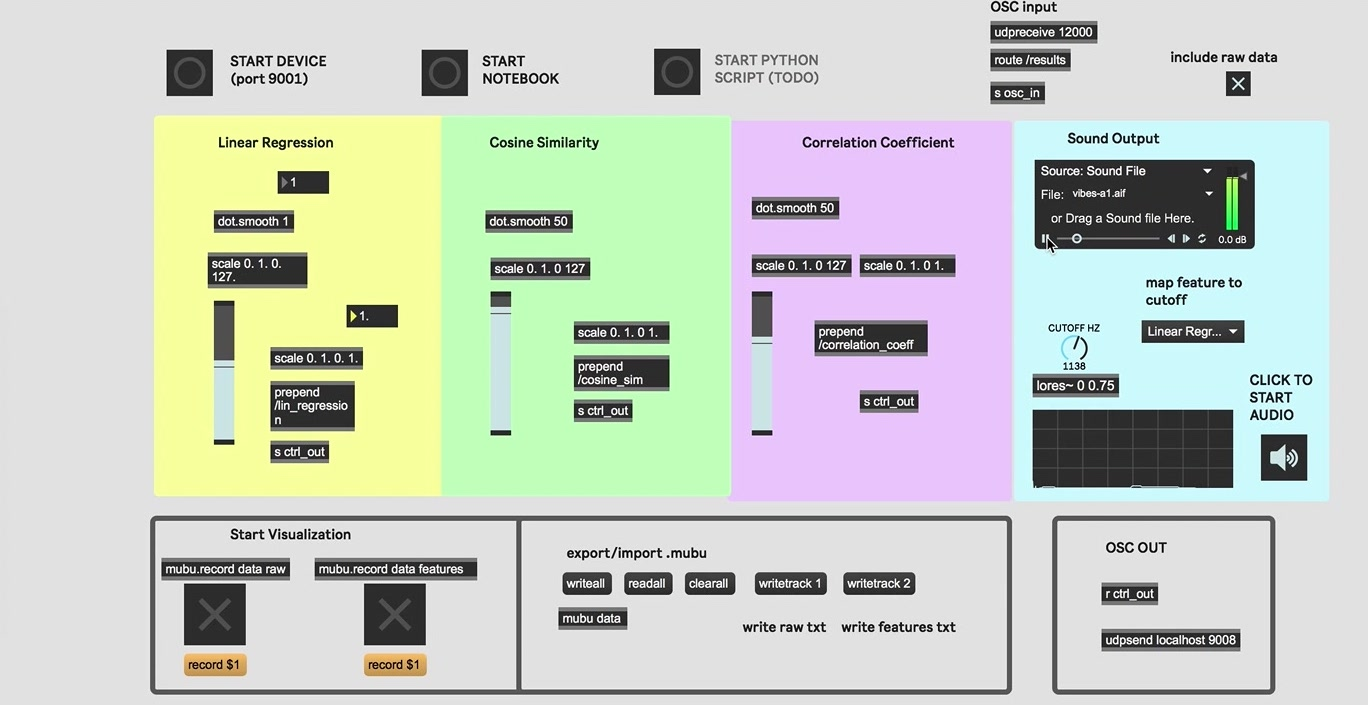
\includegraphics[width=0.8\textwidth]{Chapters/Figures/preliminary_actions/biosignals_actuation/Feature_Extraction_Sync_MAX.jpg}
\caption{Feature extraction GUI for synchrony metrics.}
\label{fig:feature_extraction_GUI}
\end{figure}

% \subsection*{Inflatable Shapes, Early Progressions}
%
% The first iteration of inflatable shapes had difficulties with fast deflation. This was partly solved by adding another air pump, devoted specifically for exhausting air. Experimenting with the addition of separators inside an inflatable shape or splitting it into multiple inflatable sections may further improve exhaust performance. Another limitation is unavoidable minor air leakage, which will happen due to imperfections in manufacturing the actuator (sealing inflatable shape, valve timing).

% \subsection*{Machine Learning and Physiological Sense-Making}
%
% A relevant part of the research presented here has focused on the extension of biosignal feature extraction, processing, and real-time analysis (e.g. to potentially enrich real-time feedback possibilities within the lab and in more ecological settings). An novel aspect in this research, is the possibility to address machine learning interactively. This research receives the name of Interactive Machine Learning. The interest in working toward the deployment and refinement of real-time machine learning processing of information is stressed throughout the thesis. However, the interactive aspect is of relevance, not only when exploring reprogrammed effects in multi-user experiences, but also when deliberately working to alter effects and come up with novel biodata-actuation mappings. This echoes early research achievements such as Wekinator \cite{} [Fiebrink, 2011] and puts forth recent progress such as that exhibited by the Teachable Machine \cite{carney_teachable_2020}. Interactive machine learning \cite{fails_interactive_2003}, originally conceptualised as a way to correct machine learning classifications on the fly has evolved significantly. By means of tools like Wekinator or Teachable Machine-like paradigms, it is possible to define actions, classes of images, movements or gestures and link them to a classification output effect.

\subsection{Adjustment and Tweakability for User Empowerment}
% User Empowerment though customisation
We describe how embodied sensor technologies react differently in accordance with the unique biological characteristics of the body. Similarly, the perceived impact of a given actuation mechanism—as those described in Section 4—largely depends on the sensitivity to a given stimulus, as well as the natural bodily variations between different users. With this considered, we recognise the necessity to attune the system’s parameters in order to produce mappings that facilitate meaningful interactions that are not overly obtrusive. While auto-calibration mechanisms have been implemented in the previous examples, which typically define and minimum/maximum parameter ranges, we foresee an extended benefit in adopting Interactive Machine Learning (IML) \cite{fails_interactive_2003,amershi_power_2014} frameworks as means to foster perspectives respecting body pluralism. Furthermore, we set out explore the use of Interactive Machine Learning to develop novel coupling relationships that go beyond linear mappings, as well as intuitive mappings between multimodal inputs and multi-dimensional outputs. In our sound-based examples, visual programming environments heavily assisted the orchestration process. In both cases, the systems enabled users to visualise a continuous stream of mappable data in real-time, clearly exposing any unexpected behaviour that may occur (for example, with the displacement of sensor electrodes). The node-based functionality of the frameworks allowed for a coherent representation of the dataflow and signal processing steps in order of execution, less abstract compared to a code-based script. During the process of developing the system, a user interface is generated in parallel on-the-fly as each node presents a GUI element that grants the designer access to parameters such as scaling and smoothing coefficients.
% In Section X.X, a basic interface allowed users to test and compare a set of algorithms for sound mappings.
This workflow can be beneficial for rapid experimentation with a variety of parameters and signal processing techniques that influence the interactive experience. It also presents a convenient solution for fine-tuning a complete system according to the user’s experience.

\section{Summary}

In this chapter, we approached the design of sensing-actuation experiences intended for rich embodied interactions. To achieve this, we adopted first-person soma design to integrate biosignals that are commonly used in ubiquitous low-cost personal sensing together with actuation mechanisms studied in HCI. Our design exploration, giving special attention to the sentient body and acknowledging alternative ways to address affect within interaction, culminated with a coupling example, in which we demonstrate data mapping strategies between respiration and sound feedback in the context of interpersonal bodily awareness. Taking this into a broader perspective, we introduce the concept of orchestration, defining the ways in which body input-output systems and meanings are put in place, the range of mappings and how they unfold. These resources mark as a theoretical and technical foundation for much of the work presented in Chapter \ref{case_studies:soma_chi}.

% \section{Latency Assessments when Using Multiple Acquisition Sources}
%
% \subsection{Motivation and Objective}
%
% Technological advancements in the field of sensory devices have allowed the collection of various bodily signals such as Acceleration (ACC), Electrocardiogram (ECG), Electromyogram (EMG), and Electrodermal Activity (EDA) using discrete wearable devices. These data streams can be used to validate semantic emotional descriptors based on valence and arousal measurements, linked to the user’s involuntary reactions transmitted by the Autonomic Nervous System (ANS). Where researchers may need to acquire data from many sources at once, we evaluate the use of the BITalino R-IoT, a low-cost sensory device designed for monitoring physiological activity in real-time.
%
% A crucial feature we want researchers to be able to exploit is the ability to acquire and process data from multiple devices simultaneously. This can be configured to monitor the activity of many users or even to place sensors on additional body parts (to track movement from different limbs, for example). To benchmark the hardware capabilities of the device in experimental environments, we carry out tests to evaluate performance, outlining the absolute and relative latency in different conditions. These tests consider the effect of including additional devices to the network and differences in wireless range of data transmission.
%
% \subsection{Preliminary Results}
%
% In our tests, we calculate the time taken for the host computer to receive a response to a stimulus which changes in the analog input on the R-IoT device, which continuously sends data back to the host computer over a shared Wi-Fi network using the Open Sound Control (OSC) protocol. The stimulus signal is distributed to multiple devices which are included in the network to see the effect this has on latency. In addition, tests are performed to evaluate the impact of increasing the wireless communication distance from 1 metre to 5 metres. The test is run for a duration of several minutes to assess how the latency deviates over time.
%
% Results show that as a base-latency, using one device at a placed a metre away from the wireless receiver, we calculated a mean latency of 8.9 milliseconds (ms). This increased to 10.7ms as the distance increased to 5 metres. When we included 4 devices, we saw a 1.1ms average increase in latency at 1 metre and 1.3ms at 5 metres. The average difference in latency among the devices was calculated as 3.2ms and 5.9ms respectively. The latency measurements were deemed stable over the time period of the test with no observable trend.
% % A complete analysis has been published on the BITalino R-IoT documentation page.
%
% We found a slight increase in latency when using more devices on one network and as we increased the distance. Whilst this should be taken account for data synchronisation tasks, we would consider the BITalino R-IoT to be a suitable device for studies collecting physiological data from multiple sources. Our tests also support the use of the OSC protocol for this purpose.
